% Copyright © 2012-2014 Martin Ueding <dev@martin-ueding.de>

% This is my general purpose LaTeX header file for writing German documents.
% Ideally, you include this using a simple ``% Copyright © 2012-2014 Martin Ueding <dev@martin-ueding.de>

% This is my general purpose LaTeX header file for writing German documents.
% Ideally, you include this using a simple ``% Copyright © 2012-2014 Martin Ueding <dev@martin-ueding.de>

% This is my general purpose LaTeX header file for writing German documents.
% Ideally, you include this using a simple ``\input{header.tex}`` in your main
% document and start with ``\title`` and ``\begin{document}`` afterwards.

% If you need to add additional packages, I recommend not doing this in this
% file, but in your main document. That way, you can just drop in a new
% ``header.tex`` and get all the new commands without having to merge manually.

% Since this file encorporates a CC-BY-SA fragment, this whole files is
% licensed under the CC-BY-SA license.

\documentclass[11pt, ngerman, fleqn, DIV=15, headinclude, BCOR=2cm]{scrreprt}

\usepackage{graphicx}

\setkomafont{caption}{\sffamily}
\setkomafont{captionlabel}{\usekomafont{caption}}

%%%%%%%%%%%%%%%%%%%%%%%%%%%%%%%%%%%%%%%%%%%%%%%%%%%%%%%%%%%%%%%%%%%%%%%%%%%%%%%
%                                Locale, date                                 %
%%%%%%%%%%%%%%%%%%%%%%%%%%%%%%%%%%%%%%%%%%%%%%%%%%%%%%%%%%%%%%%%%%%%%%%%%%%%%%%

\usepackage{babel}
\usepackage[iso]{isodate}

%%%%%%%%%%%%%%%%%%%%%%%%%%%%%%%%%%%%%%%%%%%%%%%%%%%%%%%%%%%%%%%%%%%%%%%%%%%%%%%
%                          Margins and other spacing                          %
%%%%%%%%%%%%%%%%%%%%%%%%%%%%%%%%%%%%%%%%%%%%%%%%%%%%%%%%%%%%%%%%%%%%%%%%%%%%%%%

\usepackage[parfill]{parskip}
\usepackage{setspace}
\usepackage[activate]{microtype}

\setlength{\columnsep}{2cm}

%%%%%%%%%%%%%%%%%%%%%%%%%%%%%%%%%%%%%%%%%%%%%%%%%%%%%%%%%%%%%%%%%%%%%%%%%%%%%%%
%                                    Color                                    %
%%%%%%%%%%%%%%%%%%%%%%%%%%%%%%%%%%%%%%%%%%%%%%%%%%%%%%%%%%%%%%%%%%%%%%%%%%%%%%%

\usepackage[usenames, dvipsnames]{xcolor}

\colorlet{darkred}{red!70!black}
\colorlet{darkblue}{blue!70!black}
\colorlet{darkgreen}{green!40!black}

%%%%%%%%%%%%%%%%%%%%%%%%%%%%%%%%%%%%%%%%%%%%%%%%%%%%%%%%%%%%%%%%%%%%%%%%%%%%%%%
%                         Font and font like settings                         %
%%%%%%%%%%%%%%%%%%%%%%%%%%%%%%%%%%%%%%%%%%%%%%%%%%%%%%%%%%%%%%%%%%%%%%%%%%%%%%%

% This replaces all fonts with Bitstream Charter, Bitstream Vera Sans and
% Bitstream Vera Mono. Math will be rendered in Charter.
\usepackage[charter, greekuppercase=italicized]{mathdesign}
\usepackage{beramono}
\usepackage{berasans}

% Bold, sans-serif tensors. This fragment is taken from “egreg” from
% http://tex.stackexchange.com/a/82747/8945 and licensed under `CC-BY-SA
% <https://creativecommons.org/licenses/by-sa/3.0/>`_.
\usepackage{bm}
\DeclareMathAlphabet{\mathsfit}{\encodingdefault}{\sfdefault}{m}{sl}
\SetMathAlphabet{\mathsfit}{bold}{\encodingdefault}{\sfdefault}{bx}{sl}
\newcommand{\tens}[1]{\bm{\mathsfit{#1}}}

% Bold vectors.
\renewcommand{\vec}[1]{\boldsymbol{#1}}

%%%%%%%%%%%%%%%%%%%%%%%%%%%%%%%%%%%%%%%%%%%%%%%%%%%%%%%%%%%%%%%%%%%%%%%%%%%%%%%
%                               Input encoding                                %
%%%%%%%%%%%%%%%%%%%%%%%%%%%%%%%%%%%%%%%%%%%%%%%%%%%%%%%%%%%%%%%%%%%%%%%%%%%%%%%

\usepackage[T1]{fontenc}
\usepackage[utf8]{inputenc}

%%%%%%%%%%%%%%%%%%%%%%%%%%%%%%%%%%%%%%%%%%%%%%%%%%%%%%%%%%%%%%%%%%%%%%%%%%%%%%%
%                         Hyperrefs and PDF metadata                          %
%%%%%%%%%%%%%%%%%%%%%%%%%%%%%%%%%%%%%%%%%%%%%%%%%%%%%%%%%%%%%%%%%%%%%%%%%%%%%%%

\usepackage{hyperref}

% This sets the author in the properties of the PDF as well. If you want to
% change it, just override it with another ``\hypersetup`` call.
\hypersetup{
    breaklinks=false,
    citecolor=darkgreen,
    colorlinks=true,
    linkcolor=darkblue,
    menucolor=black,
    pdfauthor={Martin Ueding},
    urlcolor=darkblue,
}

%%%%%%%%%%%%%%%%%%%%%%%%%%%%%%%%%%%%%%%%%%%%%%%%%%%%%%%%%%%%%%%%%%%%%%%%%%%%%%%
%                               Math Operators                                %
%%%%%%%%%%%%%%%%%%%%%%%%%%%%%%%%%%%%%%%%%%%%%%%%%%%%%%%%%%%%%%%%%%%%%%%%%%%%%%%

% AMS environments like ``align`` and theorems like ``proof``.
\usepackage{amsmath}
\usepackage{amsthm}

% Common math constructs like partial derivatives.
\usepackage{commath}

% Physical units.
\usepackage[output-decimal-marker={,}]{siunitx}

% Since I use mathdesign with italic uppercase greek characters, the Ohm unit will be displayed with an italic Ω by default. Units have to be roman, so this forces it the right way.
\DeclareSIUnit{\ohm}{$\Omegaup$}
\DeclareSIUnit{\division}{DIV}
\DeclareSIUnit{\voltss}{$\mathrm{V_{SS}}$}

% Word like operators.
\DeclareMathOperator{\acosh}{arcosh}
\DeclareMathOperator{\arcosh}{arcosh}
\DeclareMathOperator{\arcsinh}{arsinh}
\DeclareMathOperator{\arsinh}{arsinh}
\DeclareMathOperator{\asinh}{arsinh}
\DeclareMathOperator{\card}{card}
\DeclareMathOperator{\csch}{csch}
\DeclareMathOperator{\diam}{diam}
\DeclareMathOperator{\sech}{sech}
\renewcommand{\Im}{\mathop{{}\mathrm{Im}}\nolimits}
\renewcommand{\Re}{\mathop{{}\mathrm{Re}}\nolimits}

% Fourier transform.
\DeclareMathOperator{\fourier}{\ensuremath{\mathcal{F}}}

% Roman versions of “e” and “i” to serve as Euler's number and the imaginary
% constant.
\newcommand{\eup}{\mathrm e}
\newcommand{\iup}{\mathrm i}

% Symbols for the various mathematical fields (natural numbers, integers,
% rational numbers, real numbers, complex numbers).
\newcommand{\C}{\ensuremath{\mathbb C}}
\newcommand{\N}{\ensuremath{\mathbb N}}
\newcommand{\Q}{\ensuremath{\mathbb Q}}
\newcommand{\R}{\ensuremath{\mathbb R}}
\newcommand{\Z}{\ensuremath{\mathbb Z}}

% Shape like operators.
\DeclareMathOperator{\dalambert}{\Box}
\DeclareMathOperator{\laplace}{\bigtriangleup}
\newcommand{\curl}{\vnabla \times}
\newcommand{\divergence}[1]{\inner{\vnabla}{#1}}
\newcommand{\Divergence}[1]{\Inner{\vnabla}{#1}}
\newcommand{\vnabla}{\vec \nabla}

\newcommand{\half}{\frac 12}

% Unit vector (German „Einheitsvektor“).
\newcommand{\ev}{\hat{\vec e}}

% Mathematician's notation for the inner (scalar, dot) product.
\newcommand{\bracket}[1]{\langle #1 \rangle}
\newcommand{\Bracket}[1]{\left\langle #1 \right\rangle}
\newcommand{\inner}[2]{\bracket{#1, #2}}
\newcommand{\Inner}[2]{\Bracket{#1, #2}}

% Placeholders.
\newcommand{\fehlt}{\textcolor{darkred}{Hier fehlen noch Inhalte.}}
\newcommand{\messwert}{\textcolor{blue}{\square}}
\newcommand{\punkte}{\phantom{xxxxx}}

% Separator for equations on a single line.
\newcommand{\eqnsep}{,\quad}

% Quantum Mechanics.
\usepackage{braket}

% Thermodynamic partial derivative.
\newcommand\tdpd[3]{\del{\dpd{#1}{#2}}_{#3}}

%%%%%%%%%%%%%%%%%%%%%%%%%%%%%%%%%%%%%%%%%%%%%%%%%%%%%%%%%%%%%%%%%%%%%%%%%%%%%%%
%                                  Headings                                   %
%%%%%%%%%%%%%%%%%%%%%%%%%%%%%%%%%%%%%%%%%%%%%%%%%%%%%%%%%%%%%%%%%%%%%%%%%%%%%%%

% This will set fancy headings to the top of the page. The page number will be
% accompanied by the total number of pages. That way, you will know if any page
% is missing.
%
% If you do not want this for your document, you can just use
% ``\pagestyle{plain}``.

\usepackage{scrpage2}

\pagestyle{scrheadings}
\automark{section}
\chead{}
\ihead{}
\ohead{\rightmark}
\setheadsepline{.4pt}

%%%%%%%%%%%%%%%%%%%%%%%%%%%%%%%%%%%%%%%%%%%%%%%%%%%%%%%%%%%%%%%%%%%%%%%%%%%%%%%
%                            Bibliography (BibTeX)                            %
%%%%%%%%%%%%%%%%%%%%%%%%%%%%%%%%%%%%%%%%%%%%%%%%%%%%%%%%%%%%%%%%%%%%%%%%%%%%%%%

\newcommand{\bibliographyfile}{../../central-bibtex/Central}

\usepackage[
    backend=bibtex,
    style=alphabetic,
    %isbn=false,
    %pagetracker=false,
    %maxbibnames=50,
    %maxcitenames=2,
    %autocite=inline,
    %block=space,
    %backref=false,
    %backrefstyle=three+,
    %date=short,
    hyperref=true
]{biblatex}

\setlength{\bibitemsep}{.7em}
\setlength{\bibhang}{4ex}

\IfFileExists{\bibliographyfile}{
    \bibliography{\bibliographyfile}
}{}

%%%%%%%%%%%%%%%%%%%%%%%%%%%%%%%%%%%%%%%%%%%%%%%%%%%%%%%%%%%%%%%%%%%%%%%%%%%%%%%
%                                Abbreviations                                %
%%%%%%%%%%%%%%%%%%%%%%%%%%%%%%%%%%%%%%%%%%%%%%%%%%%%%%%%%%%%%%%%%%%%%%%%%%%%%%%

\newcommand{\dhabk}{\mbox{d.\,h.}}

%%%%%%%%%%%%%%%%%%%%%%%%%%%%%%%%%%%%%%%%%%%%%%%%%%%%%%%%%%%%%%%%%%%%%%%%%%%%%%%
%                                  Licences                                   %
%%%%%%%%%%%%%%%%%%%%%%%%%%%%%%%%%%%%%%%%%%%%%%%%%%%%%%%%%%%%%%%%%%%%%%%%%%%%%%%

\usepackage{ccicons}

\newcommand{\ccbysadetext}{%
    \begin{small}
        Dieses Werk bzw. Inhalt steht unter einer
        \href{http://creativecommons.org/licenses/by-sa/3.0/deed.de}{%
            Creative Commons Namensnennung - Weitergabe unter gleichen
        Bedingungen 3.0 Unported Lizenz}.
    \end{small}
}

\newcommand{\ccbysadetitle}{%
    Lizenz: \href{http://creativecommons.org/licenses/by-sa/3.0/deed.de}
    {CC-BY-SA 3.0 \ccbysa}
}

\newcommand\erklaerungFehlerNotation{%
    In dieser Notation bedeutet \num{1.234 +- 0.005}, dass der Wert
    $\num{1.234} \pm \num{0.005}$ ist. Die Ziffern in Klammern sind die
    Fehlerangabe. Um den Fehler zu erhalten, wird diese von rechts über die
    Zahl gelegt, alle anderen Stellen werden auf 0 gesetzt.
}

`` in your main
% document and start with ``\title`` and ``\begin{document}`` afterwards.

% If you need to add additional packages, I recommend not doing this in this
% file, but in your main document. That way, you can just drop in a new
% ``header.tex`` and get all the new commands without having to merge manually.

% Since this file encorporates a CC-BY-SA fragment, this whole files is
% licensed under the CC-BY-SA license.

\documentclass[11pt, ngerman, fleqn, DIV=15, headinclude, BCOR=2cm]{scrreprt}

\usepackage{graphicx}

\setkomafont{caption}{\sffamily}
\setkomafont{captionlabel}{\usekomafont{caption}}

%%%%%%%%%%%%%%%%%%%%%%%%%%%%%%%%%%%%%%%%%%%%%%%%%%%%%%%%%%%%%%%%%%%%%%%%%%%%%%%
%                                Locale, date                                 %
%%%%%%%%%%%%%%%%%%%%%%%%%%%%%%%%%%%%%%%%%%%%%%%%%%%%%%%%%%%%%%%%%%%%%%%%%%%%%%%

\usepackage{babel}
\usepackage[iso]{isodate}

%%%%%%%%%%%%%%%%%%%%%%%%%%%%%%%%%%%%%%%%%%%%%%%%%%%%%%%%%%%%%%%%%%%%%%%%%%%%%%%
%                          Margins and other spacing                          %
%%%%%%%%%%%%%%%%%%%%%%%%%%%%%%%%%%%%%%%%%%%%%%%%%%%%%%%%%%%%%%%%%%%%%%%%%%%%%%%

\usepackage[parfill]{parskip}
\usepackage{setspace}
\usepackage[activate]{microtype}

\setlength{\columnsep}{2cm}

%%%%%%%%%%%%%%%%%%%%%%%%%%%%%%%%%%%%%%%%%%%%%%%%%%%%%%%%%%%%%%%%%%%%%%%%%%%%%%%
%                                    Color                                    %
%%%%%%%%%%%%%%%%%%%%%%%%%%%%%%%%%%%%%%%%%%%%%%%%%%%%%%%%%%%%%%%%%%%%%%%%%%%%%%%

\usepackage[usenames, dvipsnames]{xcolor}

\colorlet{darkred}{red!70!black}
\colorlet{darkblue}{blue!70!black}
\colorlet{darkgreen}{green!40!black}

%%%%%%%%%%%%%%%%%%%%%%%%%%%%%%%%%%%%%%%%%%%%%%%%%%%%%%%%%%%%%%%%%%%%%%%%%%%%%%%
%                         Font and font like settings                         %
%%%%%%%%%%%%%%%%%%%%%%%%%%%%%%%%%%%%%%%%%%%%%%%%%%%%%%%%%%%%%%%%%%%%%%%%%%%%%%%

% This replaces all fonts with Bitstream Charter, Bitstream Vera Sans and
% Bitstream Vera Mono. Math will be rendered in Charter.
\usepackage[charter, greekuppercase=italicized]{mathdesign}
\usepackage{beramono}
\usepackage{berasans}

% Bold, sans-serif tensors. This fragment is taken from “egreg” from
% http://tex.stackexchange.com/a/82747/8945 and licensed under `CC-BY-SA
% <https://creativecommons.org/licenses/by-sa/3.0/>`_.
\usepackage{bm}
\DeclareMathAlphabet{\mathsfit}{\encodingdefault}{\sfdefault}{m}{sl}
\SetMathAlphabet{\mathsfit}{bold}{\encodingdefault}{\sfdefault}{bx}{sl}
\newcommand{\tens}[1]{\bm{\mathsfit{#1}}}

% Bold vectors.
\renewcommand{\vec}[1]{\boldsymbol{#1}}

%%%%%%%%%%%%%%%%%%%%%%%%%%%%%%%%%%%%%%%%%%%%%%%%%%%%%%%%%%%%%%%%%%%%%%%%%%%%%%%
%                               Input encoding                                %
%%%%%%%%%%%%%%%%%%%%%%%%%%%%%%%%%%%%%%%%%%%%%%%%%%%%%%%%%%%%%%%%%%%%%%%%%%%%%%%

\usepackage[T1]{fontenc}
\usepackage[utf8]{inputenc}

%%%%%%%%%%%%%%%%%%%%%%%%%%%%%%%%%%%%%%%%%%%%%%%%%%%%%%%%%%%%%%%%%%%%%%%%%%%%%%%
%                         Hyperrefs and PDF metadata                          %
%%%%%%%%%%%%%%%%%%%%%%%%%%%%%%%%%%%%%%%%%%%%%%%%%%%%%%%%%%%%%%%%%%%%%%%%%%%%%%%

\usepackage{hyperref}

% This sets the author in the properties of the PDF as well. If you want to
% change it, just override it with another ``\hypersetup`` call.
\hypersetup{
    breaklinks=false,
    citecolor=darkgreen,
    colorlinks=true,
    linkcolor=darkblue,
    menucolor=black,
    pdfauthor={Martin Ueding},
    urlcolor=darkblue,
}

%%%%%%%%%%%%%%%%%%%%%%%%%%%%%%%%%%%%%%%%%%%%%%%%%%%%%%%%%%%%%%%%%%%%%%%%%%%%%%%
%                               Math Operators                                %
%%%%%%%%%%%%%%%%%%%%%%%%%%%%%%%%%%%%%%%%%%%%%%%%%%%%%%%%%%%%%%%%%%%%%%%%%%%%%%%

% AMS environments like ``align`` and theorems like ``proof``.
\usepackage{amsmath}
\usepackage{amsthm}

% Common math constructs like partial derivatives.
\usepackage{commath}

% Physical units.
\usepackage[output-decimal-marker={,}]{siunitx}

% Since I use mathdesign with italic uppercase greek characters, the Ohm unit will be displayed with an italic Ω by default. Units have to be roman, so this forces it the right way.
\DeclareSIUnit{\ohm}{$\Omegaup$}
\DeclareSIUnit{\division}{DIV}
\DeclareSIUnit{\voltss}{$\mathrm{V_{SS}}$}

% Word like operators.
\DeclareMathOperator{\acosh}{arcosh}
\DeclareMathOperator{\arcosh}{arcosh}
\DeclareMathOperator{\arcsinh}{arsinh}
\DeclareMathOperator{\arsinh}{arsinh}
\DeclareMathOperator{\asinh}{arsinh}
\DeclareMathOperator{\card}{card}
\DeclareMathOperator{\csch}{csch}
\DeclareMathOperator{\diam}{diam}
\DeclareMathOperator{\sech}{sech}
\renewcommand{\Im}{\mathop{{}\mathrm{Im}}\nolimits}
\renewcommand{\Re}{\mathop{{}\mathrm{Re}}\nolimits}

% Fourier transform.
\DeclareMathOperator{\fourier}{\ensuremath{\mathcal{F}}}

% Roman versions of “e” and “i” to serve as Euler's number and the imaginary
% constant.
\newcommand{\eup}{\mathrm e}
\newcommand{\iup}{\mathrm i}

% Symbols for the various mathematical fields (natural numbers, integers,
% rational numbers, real numbers, complex numbers).
\newcommand{\C}{\ensuremath{\mathbb C}}
\newcommand{\N}{\ensuremath{\mathbb N}}
\newcommand{\Q}{\ensuremath{\mathbb Q}}
\newcommand{\R}{\ensuremath{\mathbb R}}
\newcommand{\Z}{\ensuremath{\mathbb Z}}

% Shape like operators.
\DeclareMathOperator{\dalambert}{\Box}
\DeclareMathOperator{\laplace}{\bigtriangleup}
\newcommand{\curl}{\vnabla \times}
\newcommand{\divergence}[1]{\inner{\vnabla}{#1}}
\newcommand{\Divergence}[1]{\Inner{\vnabla}{#1}}
\newcommand{\vnabla}{\vec \nabla}

\newcommand{\half}{\frac 12}

% Unit vector (German „Einheitsvektor“).
\newcommand{\ev}{\hat{\vec e}}

% Mathematician's notation for the inner (scalar, dot) product.
\newcommand{\bracket}[1]{\langle #1 \rangle}
\newcommand{\Bracket}[1]{\left\langle #1 \right\rangle}
\newcommand{\inner}[2]{\bracket{#1, #2}}
\newcommand{\Inner}[2]{\Bracket{#1, #2}}

% Placeholders.
\newcommand{\fehlt}{\textcolor{darkred}{Hier fehlen noch Inhalte.}}
\newcommand{\messwert}{\textcolor{blue}{\square}}
\newcommand{\punkte}{\phantom{xxxxx}}

% Separator for equations on a single line.
\newcommand{\eqnsep}{,\quad}

% Quantum Mechanics.
\usepackage{braket}

% Thermodynamic partial derivative.
\newcommand\tdpd[3]{\del{\dpd{#1}{#2}}_{#3}}

%%%%%%%%%%%%%%%%%%%%%%%%%%%%%%%%%%%%%%%%%%%%%%%%%%%%%%%%%%%%%%%%%%%%%%%%%%%%%%%
%                                  Headings                                   %
%%%%%%%%%%%%%%%%%%%%%%%%%%%%%%%%%%%%%%%%%%%%%%%%%%%%%%%%%%%%%%%%%%%%%%%%%%%%%%%

% This will set fancy headings to the top of the page. The page number will be
% accompanied by the total number of pages. That way, you will know if any page
% is missing.
%
% If you do not want this for your document, you can just use
% ``\pagestyle{plain}``.

\usepackage{scrpage2}

\pagestyle{scrheadings}
\automark{section}
\chead{}
\ihead{}
\ohead{\rightmark}
\setheadsepline{.4pt}

%%%%%%%%%%%%%%%%%%%%%%%%%%%%%%%%%%%%%%%%%%%%%%%%%%%%%%%%%%%%%%%%%%%%%%%%%%%%%%%
%                            Bibliography (BibTeX)                            %
%%%%%%%%%%%%%%%%%%%%%%%%%%%%%%%%%%%%%%%%%%%%%%%%%%%%%%%%%%%%%%%%%%%%%%%%%%%%%%%

\newcommand{\bibliographyfile}{../../central-bibtex/Central}

\usepackage[
    backend=bibtex,
    style=alphabetic,
    %isbn=false,
    %pagetracker=false,
    %maxbibnames=50,
    %maxcitenames=2,
    %autocite=inline,
    %block=space,
    %backref=false,
    %backrefstyle=three+,
    %date=short,
    hyperref=true
]{biblatex}

\setlength{\bibitemsep}{.7em}
\setlength{\bibhang}{4ex}

\IfFileExists{\bibliographyfile}{
    \bibliography{\bibliographyfile}
}{}

%%%%%%%%%%%%%%%%%%%%%%%%%%%%%%%%%%%%%%%%%%%%%%%%%%%%%%%%%%%%%%%%%%%%%%%%%%%%%%%
%                                Abbreviations                                %
%%%%%%%%%%%%%%%%%%%%%%%%%%%%%%%%%%%%%%%%%%%%%%%%%%%%%%%%%%%%%%%%%%%%%%%%%%%%%%%

\newcommand{\dhabk}{\mbox{d.\,h.}}

%%%%%%%%%%%%%%%%%%%%%%%%%%%%%%%%%%%%%%%%%%%%%%%%%%%%%%%%%%%%%%%%%%%%%%%%%%%%%%%
%                                  Licences                                   %
%%%%%%%%%%%%%%%%%%%%%%%%%%%%%%%%%%%%%%%%%%%%%%%%%%%%%%%%%%%%%%%%%%%%%%%%%%%%%%%

\usepackage{ccicons}

\newcommand{\ccbysadetext}{%
    \begin{small}
        Dieses Werk bzw. Inhalt steht unter einer
        \href{http://creativecommons.org/licenses/by-sa/3.0/deed.de}{%
            Creative Commons Namensnennung - Weitergabe unter gleichen
        Bedingungen 3.0 Unported Lizenz}.
    \end{small}
}

\newcommand{\ccbysadetitle}{%
    Lizenz: \href{http://creativecommons.org/licenses/by-sa/3.0/deed.de}
    {CC-BY-SA 3.0 \ccbysa}
}

\newcommand\erklaerungFehlerNotation{%
    In dieser Notation bedeutet \num{1.234 +- 0.005}, dass der Wert
    $\num{1.234} \pm \num{0.005}$ ist. Die Ziffern in Klammern sind die
    Fehlerangabe. Um den Fehler zu erhalten, wird diese von rechts über die
    Zahl gelegt, alle anderen Stellen werden auf 0 gesetzt.
}

`` in your main
% document and start with ``\title`` and ``\begin{document}`` afterwards.

% If you need to add additional packages, I recommend not doing this in this
% file, but in your main document. That way, you can just drop in a new
% ``header.tex`` and get all the new commands without having to merge manually.

% Since this file encorporates a CC-BY-SA fragment, this whole files is
% licensed under the CC-BY-SA license.

\documentclass[11pt, ngerman, fleqn, DIV=15, headinclude, BCOR=2cm]{scrreprt}

\usepackage{graphicx}

\setkomafont{caption}{\sffamily}
\setkomafont{captionlabel}{\usekomafont{caption}}

%%%%%%%%%%%%%%%%%%%%%%%%%%%%%%%%%%%%%%%%%%%%%%%%%%%%%%%%%%%%%%%%%%%%%%%%%%%%%%%
%                                Locale, date                                 %
%%%%%%%%%%%%%%%%%%%%%%%%%%%%%%%%%%%%%%%%%%%%%%%%%%%%%%%%%%%%%%%%%%%%%%%%%%%%%%%

\usepackage{babel}
\usepackage[iso]{isodate}

%%%%%%%%%%%%%%%%%%%%%%%%%%%%%%%%%%%%%%%%%%%%%%%%%%%%%%%%%%%%%%%%%%%%%%%%%%%%%%%
%                          Margins and other spacing                          %
%%%%%%%%%%%%%%%%%%%%%%%%%%%%%%%%%%%%%%%%%%%%%%%%%%%%%%%%%%%%%%%%%%%%%%%%%%%%%%%

\usepackage[parfill]{parskip}
\usepackage{setspace}
\usepackage[activate]{microtype}

\setlength{\columnsep}{2cm}

%%%%%%%%%%%%%%%%%%%%%%%%%%%%%%%%%%%%%%%%%%%%%%%%%%%%%%%%%%%%%%%%%%%%%%%%%%%%%%%
%                                    Color                                    %
%%%%%%%%%%%%%%%%%%%%%%%%%%%%%%%%%%%%%%%%%%%%%%%%%%%%%%%%%%%%%%%%%%%%%%%%%%%%%%%

\usepackage[usenames, dvipsnames]{xcolor}

\colorlet{darkred}{red!70!black}
\colorlet{darkblue}{blue!70!black}
\colorlet{darkgreen}{green!40!black}

%%%%%%%%%%%%%%%%%%%%%%%%%%%%%%%%%%%%%%%%%%%%%%%%%%%%%%%%%%%%%%%%%%%%%%%%%%%%%%%
%                         Font and font like settings                         %
%%%%%%%%%%%%%%%%%%%%%%%%%%%%%%%%%%%%%%%%%%%%%%%%%%%%%%%%%%%%%%%%%%%%%%%%%%%%%%%

% This replaces all fonts with Bitstream Charter, Bitstream Vera Sans and
% Bitstream Vera Mono. Math will be rendered in Charter.
\usepackage[charter, greekuppercase=italicized]{mathdesign}
\usepackage{beramono}
\usepackage{berasans}

% Bold, sans-serif tensors. This fragment is taken from “egreg” from
% http://tex.stackexchange.com/a/82747/8945 and licensed under `CC-BY-SA
% <https://creativecommons.org/licenses/by-sa/3.0/>`_.
\usepackage{bm}
\DeclareMathAlphabet{\mathsfit}{\encodingdefault}{\sfdefault}{m}{sl}
\SetMathAlphabet{\mathsfit}{bold}{\encodingdefault}{\sfdefault}{bx}{sl}
\newcommand{\tens}[1]{\bm{\mathsfit{#1}}}

% Bold vectors.
\renewcommand{\vec}[1]{\boldsymbol{#1}}

%%%%%%%%%%%%%%%%%%%%%%%%%%%%%%%%%%%%%%%%%%%%%%%%%%%%%%%%%%%%%%%%%%%%%%%%%%%%%%%
%                               Input encoding                                %
%%%%%%%%%%%%%%%%%%%%%%%%%%%%%%%%%%%%%%%%%%%%%%%%%%%%%%%%%%%%%%%%%%%%%%%%%%%%%%%

\usepackage[T1]{fontenc}
\usepackage[utf8]{inputenc}

%%%%%%%%%%%%%%%%%%%%%%%%%%%%%%%%%%%%%%%%%%%%%%%%%%%%%%%%%%%%%%%%%%%%%%%%%%%%%%%
%                         Hyperrefs and PDF metadata                          %
%%%%%%%%%%%%%%%%%%%%%%%%%%%%%%%%%%%%%%%%%%%%%%%%%%%%%%%%%%%%%%%%%%%%%%%%%%%%%%%

\usepackage{hyperref}

% This sets the author in the properties of the PDF as well. If you want to
% change it, just override it with another ``\hypersetup`` call.
\hypersetup{
    breaklinks=false,
    citecolor=darkgreen,
    colorlinks=true,
    linkcolor=darkblue,
    menucolor=black,
    pdfauthor={Martin Ueding},
    urlcolor=darkblue,
}

%%%%%%%%%%%%%%%%%%%%%%%%%%%%%%%%%%%%%%%%%%%%%%%%%%%%%%%%%%%%%%%%%%%%%%%%%%%%%%%
%                               Math Operators                                %
%%%%%%%%%%%%%%%%%%%%%%%%%%%%%%%%%%%%%%%%%%%%%%%%%%%%%%%%%%%%%%%%%%%%%%%%%%%%%%%

% AMS environments like ``align`` and theorems like ``proof``.
\usepackage{amsmath}
\usepackage{amsthm}

% Common math constructs like partial derivatives.
\usepackage{commath}

% Physical units.
\usepackage[output-decimal-marker={,}]{siunitx}

% Since I use mathdesign with italic uppercase greek characters, the Ohm unit will be displayed with an italic Ω by default. Units have to be roman, so this forces it the right way.
\DeclareSIUnit{\ohm}{$\Omegaup$}
\DeclareSIUnit{\division}{DIV}
\DeclareSIUnit{\voltss}{$\mathrm{V_{SS}}$}

% Word like operators.
\DeclareMathOperator{\acosh}{arcosh}
\DeclareMathOperator{\arcosh}{arcosh}
\DeclareMathOperator{\arcsinh}{arsinh}
\DeclareMathOperator{\arsinh}{arsinh}
\DeclareMathOperator{\asinh}{arsinh}
\DeclareMathOperator{\card}{card}
\DeclareMathOperator{\csch}{csch}
\DeclareMathOperator{\diam}{diam}
\DeclareMathOperator{\sech}{sech}
\renewcommand{\Im}{\mathop{{}\mathrm{Im}}\nolimits}
\renewcommand{\Re}{\mathop{{}\mathrm{Re}}\nolimits}

% Fourier transform.
\DeclareMathOperator{\fourier}{\ensuremath{\mathcal{F}}}

% Roman versions of “e” and “i” to serve as Euler's number and the imaginary
% constant.
\newcommand{\eup}{\mathrm e}
\newcommand{\iup}{\mathrm i}

% Symbols for the various mathematical fields (natural numbers, integers,
% rational numbers, real numbers, complex numbers).
\newcommand{\C}{\ensuremath{\mathbb C}}
\newcommand{\N}{\ensuremath{\mathbb N}}
\newcommand{\Q}{\ensuremath{\mathbb Q}}
\newcommand{\R}{\ensuremath{\mathbb R}}
\newcommand{\Z}{\ensuremath{\mathbb Z}}

% Shape like operators.
\DeclareMathOperator{\dalambert}{\Box}
\DeclareMathOperator{\laplace}{\bigtriangleup}
\newcommand{\curl}{\vnabla \times}
\newcommand{\divergence}[1]{\inner{\vnabla}{#1}}
\newcommand{\Divergence}[1]{\Inner{\vnabla}{#1}}
\newcommand{\vnabla}{\vec \nabla}

\newcommand{\half}{\frac 12}

% Unit vector (German „Einheitsvektor“).
\newcommand{\ev}{\hat{\vec e}}

% Mathematician's notation for the inner (scalar, dot) product.
\newcommand{\bracket}[1]{\langle #1 \rangle}
\newcommand{\Bracket}[1]{\left\langle #1 \right\rangle}
\newcommand{\inner}[2]{\bracket{#1, #2}}
\newcommand{\Inner}[2]{\Bracket{#1, #2}}

% Placeholders.
\newcommand{\fehlt}{\textcolor{darkred}{Hier fehlen noch Inhalte.}}
\newcommand{\messwert}{\textcolor{blue}{\square}}
\newcommand{\punkte}{\phantom{xxxxx}}

% Separator for equations on a single line.
\newcommand{\eqnsep}{,\quad}

% Quantum Mechanics.
\usepackage{braket}

% Thermodynamic partial derivative.
\newcommand\tdpd[3]{\del{\dpd{#1}{#2}}_{#3}}

%%%%%%%%%%%%%%%%%%%%%%%%%%%%%%%%%%%%%%%%%%%%%%%%%%%%%%%%%%%%%%%%%%%%%%%%%%%%%%%
%                                  Headings                                   %
%%%%%%%%%%%%%%%%%%%%%%%%%%%%%%%%%%%%%%%%%%%%%%%%%%%%%%%%%%%%%%%%%%%%%%%%%%%%%%%

% This will set fancy headings to the top of the page. The page number will be
% accompanied by the total number of pages. That way, you will know if any page
% is missing.
%
% If you do not want this for your document, you can just use
% ``\pagestyle{plain}``.

\usepackage{scrpage2}

\pagestyle{scrheadings}
\automark{section}
\chead{}
\ihead{}
\ohead{\rightmark}
\setheadsepline{.4pt}

%%%%%%%%%%%%%%%%%%%%%%%%%%%%%%%%%%%%%%%%%%%%%%%%%%%%%%%%%%%%%%%%%%%%%%%%%%%%%%%
%                            Bibliography (BibTeX)                            %
%%%%%%%%%%%%%%%%%%%%%%%%%%%%%%%%%%%%%%%%%%%%%%%%%%%%%%%%%%%%%%%%%%%%%%%%%%%%%%%

\newcommand{\bibliographyfile}{../../central-bibtex/Central}

\usepackage[
    backend=bibtex,
    style=alphabetic,
    %isbn=false,
    %pagetracker=false,
    %maxbibnames=50,
    %maxcitenames=2,
    %autocite=inline,
    %block=space,
    %backref=false,
    %backrefstyle=three+,
    %date=short,
    hyperref=true
]{biblatex}

\setlength{\bibitemsep}{.7em}
\setlength{\bibhang}{4ex}

\IfFileExists{\bibliographyfile}{
    \bibliography{\bibliographyfile}
}{}

%%%%%%%%%%%%%%%%%%%%%%%%%%%%%%%%%%%%%%%%%%%%%%%%%%%%%%%%%%%%%%%%%%%%%%%%%%%%%%%
%                                Abbreviations                                %
%%%%%%%%%%%%%%%%%%%%%%%%%%%%%%%%%%%%%%%%%%%%%%%%%%%%%%%%%%%%%%%%%%%%%%%%%%%%%%%

\newcommand{\dhabk}{\mbox{d.\,h.}}

%%%%%%%%%%%%%%%%%%%%%%%%%%%%%%%%%%%%%%%%%%%%%%%%%%%%%%%%%%%%%%%%%%%%%%%%%%%%%%%
%                                  Licences                                   %
%%%%%%%%%%%%%%%%%%%%%%%%%%%%%%%%%%%%%%%%%%%%%%%%%%%%%%%%%%%%%%%%%%%%%%%%%%%%%%%

\usepackage{ccicons}

\newcommand{\ccbysadetext}{%
    \begin{small}
        Dieses Werk bzw. Inhalt steht unter einer
        \href{http://creativecommons.org/licenses/by-sa/3.0/deed.de}{%
            Creative Commons Namensnennung - Weitergabe unter gleichen
        Bedingungen 3.0 Unported Lizenz}.
    \end{small}
}

\newcommand{\ccbysadetitle}{%
    Lizenz: \href{http://creativecommons.org/licenses/by-sa/3.0/deed.de}
    {CC-BY-SA 3.0 \ccbysa}
}

\newcommand\erklaerungFehlerNotation{%
    In dieser Notation bedeutet \num{1.234 +- 0.005}, dass der Wert
    $\num{1.234} \pm \num{0.005}$ ist. Die Ziffern in Klammern sind die
    Fehlerangabe. Um den Fehler zu erhalten, wird diese von rechts über die
    Zahl gelegt, alle anderen Stellen werden auf 0 gesetzt.
}



\usepackage[section]{placeins}

\usepackage{csquotes}

\usepackage{tikz}
\usetikzlibrary{chains}
\usetikzlibrary{shapes.geometric}

\tikzset{device/.style={
                rectangle,
                minimum size=6mm,
                draw=black
            },
            monitor/.style={
                rectangle,
                rounded corners=2mm,
                minimum size=6mm,
                draw=black
            },
        }

\usepackage{pgfplots}
\pgfplotsset{
    compat=1.5,
    width=0.8\linewidth,
    xticklabel style={/pgf/number format/use comma},
    yticklabel style={/pgf/number format/use comma},
}

\usepgfplotslibrary{external}
\tikzexternalize

\DeclareSIUnit{\skt}{SKT}

\usepackage{booktabs}

\hypersetup{
    pdftitle=
}

\subject{Praktikumsprotokoll}
\title{Compton-Effekt}
\subtitle{Versuch P526 -- Universität Bonn}
\author{
    Martin Ueding \\ \small{\href{mailto:mu@martin-ueding.de}{mu@martin-ueding.de}}
    \and
    Lino Lemmer \\
    \small{\href{mailto:l2@uni-bonn.de}{l2@uni-bonn.de}}
}

\date{\daterange{2014-05-07}{2014-05-08}}

% TODO Tutor Eintragen
%\publishers{Tutor: TODO}

\begin{document}

\maketitle

\begin{abstract}
    % TODO Abstract formulieren.
\end{abstract}

\tableofcontents

\chapter{Theorie}

% TODO Sollen wir noch explizit machen, dass wir dies aus einem vorherigen
% Protokoll übernommen haben?

Aufgrund der thematischen Überschneidung mit Versuch 525, den vor bereits
durchgeführt haben, übernehmen wir einige Abschnitte aus dem Theorieteil von
\parencite{Ueding/525}.

\section{Wechselwirkung von $\gammaup$-Strahlung mit Materie}
\label{sec:WW}

Trifft $\gammaup$-Strahlung auf Materie, finden abhängig von Photonenergie und
Ordnungszahl des Atoms unterschiedliche Effekte statt.

\subsection{Photoeffekt}

Als Photoeffekt, auch photoelektrischer oder lichtelektrischer Effekt,
bezeichnet man den Prozess, bei dem ein Photon seine gesamte Energie an ein
Elektron abgibt. Ist diese Energie größer als die Bindungsenergie des
Elektrons, wird dieses aus seiner Bindung gelöst. Die dadurch entstehenden
freien Stellen werden durch höherenergetische Elektronen wieder gefüllt, wobei
sie Photonen emittieren.

% TODO Abhängigkeit des Wirkungsquerschnittes von E.

\subsection{Paarbildung}

Zerfällt ein Photon im Coulombfeld eines Atomkerns in ein
Elektron-Positron-Paar, spricht man von einer Paarbildung. Dies kann nur
stattfinden, wenn die Energie des Photons die Ruheenergie der beiden Teilchen
übersteigt, also $E_\gammaup > 2m_\mathrm{e}c^2$. Zudem findet es bevorzugt bei
hohen Ordnungszahlen statt, da dort die Divergenz des Feldes größer ist.

% TODO Abhängigkeit des Wirkungsquerschnittes von E.

\subsection{Compton-Streuung}

Als Compton-Streuung bezeichnet man die elastische Streuung von Photonen zum
Beispiel an Elektronen. Die dabei vom Photon an das Elektron übertragene
Energie hängt nur vom Winkel ab und ist Maximal bei einem Streuwinkel von $\phi
= \SI{180}\degree$, also bei einer Rückstreuung, und minimal bei $\phi =
\SI{0}\degree$, also wenn das Elektron nur gestreift wird.

Werden nun viele Photonen mit einer Energie $E_\nu$ gestreut, wie es in einem
Szintillator der Fall ist, ergibt sich ein charakteristisches Bild. In
Abbildung~\ref{fig:Compton} ist idealisiert die Intensität gegen die an den
Szintillator übertragene Energie dargestellt. Das Compton-Kontinuum entsteht
durch die Streuung mit unterschiedlichen Winkeln, die Compton-Kante wird durch
den maximalen Energieübertrag bei $\phi = \SI{180}{\degree}$ erzeugt. Der
Photopeak, oder auch Full-Energy-Peak bei $E_\nu$ entsteht durch die
vollständige Deponierung der Photonenergie im Szintillator, beispielsweise
durch den Photoeffekt. Die Restenergie des zurück gestreuten Photons ist genau
die Differenz von $E_\nu$ und der Energie an der Compton-Kante.

\begin{figure}[htbp]
    \centering
    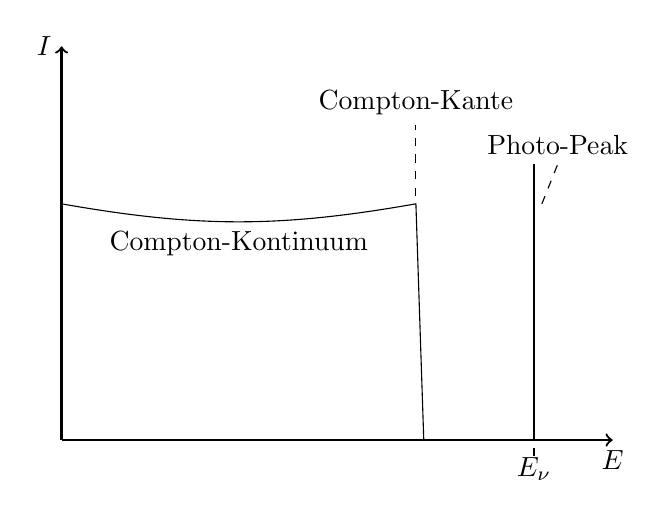
\begin{tikzpicture}
        \draw[thick,->]
        (0,0) -- (0,5) node[left] {$I$}
        ;
        \draw[thick,->]
        (0,0) -- (7,0) node[below] {$E$}
        ;
        \draw
        (6,0) -- (6,3.5)
        ;
        \draw
        (6,-.2) -- (6,-.1) node[below] {$E_\nu$}
        ;
        \draw[bend right=10]
        (0,3) to node[below] {Compton-Kontinuum} (4.5,3) -- (4.6,0)
        ;
        \draw[dashed]
        (4.5,3.1) -- (4.5,4) node[above] {Compton-Kante}
        ;
        \draw[dashed]
        (6.1,3) -- (6.3,3.5) node[above] {Photo-Peak}
        ;
    \end{tikzpicture}
    \caption{%
        Idealisiertes Spektrum der bei Einstrahlung von monochromatischer
        $\gammaup$-Strahlung an den Szintillator übertragenen Energie
    }
    \label{fig:Compton}
\end{figure}


% TODO Compton Streuformel.

% TODO Compton Wellenlänge.

\subsubsection{Differentieller Wirkungsquerschnitt}

Die Klein-Nishina Formel wurde aus der QFT hergeleitet und ist
\parencite[(2.107)]{Leo/Techniques_Nuclear_Experiments}
\[
    \dod\sigma\Omega =
    \frac{r_\text e^2}2 \frac1{\del{1 + \gamma(1 - \cos(\theta))}^2}
    \del{
        1 + \cos(\theta)^2 + \frac{\gamma^2(1 - \cos(\theta)^2)}{1 + \gamma(1 -
        \cos(\theta))}
    }.
\]
Sie beschreibt den differentiellen Wirkungsquerschnitt der Compton-Streuuung in
Abhängigkeit der Energie ($\gamma := h\nu / m_\text e c^2$) und des
Polarwinkels $\theta$.

% TODO Klein-Nishina-Plot.

\subsubsection{Totaler Stoßwirkungsquerschnitt}

Durch Integration des differentiellen Wirkungsquerschnitts nach dem Raumwinkel
erhält man den totalen Wirkungsquerschnitt. Dieser ist in
\parencite[(2.107)]{Leo/Techniques_Nuclear_Experiments} gegeben als
\[
    \sigma = 2 \piup r_\text e^2 \del{
        \frac{1+\gamma}{\gamma^2} \del{
            \frac{2(1+\gamma)}{1+2\gamma} - \frac1\gamma \ln(1+2\gamma)
        }
        + \frac1{2\gamma} \ln(1+2\gamma) - \frac{1+3\gamma}{(1+2\gamma)^2}
    }.
\]

\subsubsection{Abhängigkeit des Wirkungsquerschnitts von $E_\nu$}

Mit $s := T / h \nu$ lässt sich aus der Klein-Nishina Formel das
Energiespektrum herleiten
\parencite[(2.113)]{Leo/Techniques_Nuclear_Experiments}:
\[
    \dod\sigmaT =
    \frac{\piup r_\text e^2}{m_\text e c^2 \gamma^2} \del{
        2 + \frac{s^2}{\gamma^2(1 - s)^2} + \frac{s}{1-s} \del{
            s - \frac2\gamma
        }
    }
\]

Im Fall von $\theta = \piup$ wird der meiste Impuls und Energie auf das
Elektron übertragen. Diese Maximalenergie zeigt sich im Spektrum als
„Comptonkante“ und ist gegeben durch
\parencite[(2.114)]{Leo/Techniques_Nuclear_Experiments}
\[
    T_\text{max} = h \nu \frac{2\gamma}{1+2\gamma}.
\]



% TODO Linearpolarisation von γ-Quanten.

% TODO Abschwächung von γ-Strahlung in Materie.

% TODO totaler Abschwächungskoeffizient.

\subsection{Thomsonstreuung}

Die Thomsonstreuung ist der niederenergetische Grenzfall der Comptonstreuung.
In diesem Fall wird keine Energie an das Elektron übertragen. Dadurch sind
diese Effekte nur dafür verantwortlich, dass die Ausbreitungsrichtung der
Photonen geändert wird. Ist die Photonenenergie deutlich kleiner als die
Elektronenmasse, so vereinfacht sich die Klein-Nishina-Formel zu
\parencite[(2.115)]{Leo/Techniques_Nuclear_Experiments}
\[
    \sigma = \frac{8\piup}3 r_\text e^2.
\]

\subsection{Rückstreu- und Escape-Peak}

Wird ein Photon, nachdem es durch den Compton-Effekt zurückgeworfen wurde, ein
weiteres Mal um $\phi = \SI{180}{\degree}$ gestreut, oder in einem
gegenüberliegenden Szintillator detektiert, entsteht ein weiterer Peak, der
eine Spektrallinie vortäuscht. Dies ist der Rückstreu-Peak. Die Energie dieses
Peaks ist daher identisch mit der Restenergie des Photons.

Kommt es zur Paarbildung, wird nur dann die volle Energie im Szintillator
deponiert, wenn das entstehende Positron auf ein Elektron trifft, unter Abgabe
zweier \SI{511}{\kilo\electronvolt}-Photonen annihilliert und beide
entstehenden Photonen durch andere Effekte ihre Energie an den Szintillator
abgeben. Verlässt eines der Photonen oder sogar beide den Szintillator, ohne
Energie abzugeben, entsteht eine weitere scheinbare Spektrallinie, der Single-
bzw. Double-Escape-Peak, bei einer Energie von
$E_\nu-\SI{511}{\kilo\electronvolt}$ bzw. $E_\nu-\SI{1022}{\kilo\electronvolt}$.

% TODO Form des Spektrums.

% TODO Peak to Total Verhältnis.

\section{Instrumente}

\subsection{Szintillator}

Zur Detektion von $\gammaup$-Quanten verwendet man einen Kristall, zum Beispiel
Natriumiodid. Trifft nun ein $\gammaup$ auf ein Elektron, wird es durch die
Effekte aus \ref{sec:WW} angeregt. Bei einer Abregung über Zwischenniveaus
werden Photonen niedrigerer Energie abgegeben, welche von einem
Photomultiplier eingefangen werden können. Eine andere Möglichkeit ist der
Stoß mit anderen Elektronen, wodurch zwei Elektronen mit geringerer Energie
entstehen. Die Intensität des Lichtblitzes ist dabei proportional zur Energie
des ursprünglichen $\gammaup$-Quants.

% TODO Energieauflösung.

% TODO Totzeit.

% TODO Selbsttransparenz.

\subsection{Photomultiplier (PM)}

Will man ein schwaches optisches Signal in eine messbares elektrisches Signal
umwandeln, benötigt man einen Photomultiplier. Ein möglicher Aufbau ist in
Abbildung~\ref{fig:PM} zu sehen. Zwischen Photokathode und Anode liegt eine
Spannung an, die von Dynode zu Dynode abfällt.

Trifft ein Photon auf die Photokathode, löst es, wenn seine Energie die
Austrittsarbeit übersteigt, ein Elektron aus dieser heraus. Durch die angelegte
Spannung wird das Elektron beschleunigt und zum Beispiel durch ein Elektrisches
Feld so abgelenkt, dass es auf die erste Dynode trifft. Hier löst es weitere
Elektronen aus, die zur nächsten Dynode beschleunigt werden. Der Prozess geht
so weiter, bis zum Schluss die Lawinenelektronen auf die Anode treffen und dort
ein messbares elektronisches Signal ergeben.

Da die Anzahl der ausgelösten Elektronen proportional zur Intensität der
eintreffenden Strahlung ist, und da der Photomultiplier linear verstärkt, ist
das Ausgangssignal proportional zur einfallenden Intensität. Wird ein
Szintillatorsignal verstärkt, ist die Amplitude also proportional zur Energie
der $\gammaup$-Strahlung.

An der Anode liegt meistens Sättigung vor. Dies sorgt dafür, dass die Amplitude
des Signals keine Aussage mehr über die Energie machen kann aber durch eine
Anstiegszeit von wenigen \si{\nano\second} eine hohe Zeitgenauigkeit erreicht
wird. Wegen des schnellen Anstiegs wird das Ausgangssignal daher auch
\emph{Fast}-Signal genannt.

Greift man das Signal an einer Dynode, an der noch keine Sättigung herrscht ab,
ist eine Aussage über die Energie des verursachenden Photons möglich. Die
Anstiegszeit ist jedoch deutlich größer. Daher heißt dieses Signal auch
\emph{Slow}-Signal.

\begin{figure}[htbp]
    \centering
    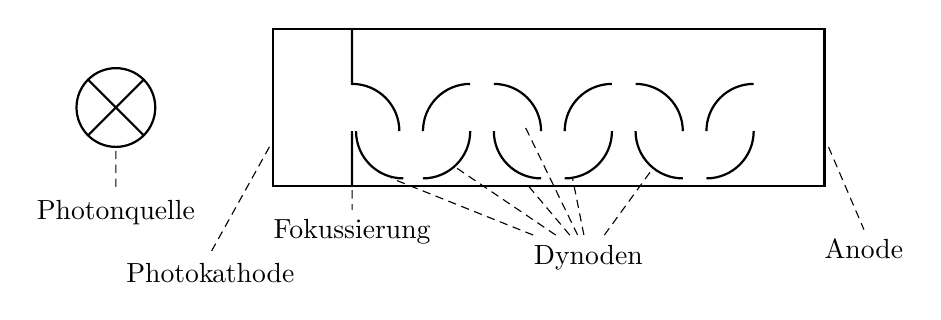
\begin{tikzpicture}
        % Röhre
        \draw[thick] (2,-1) rectangle (9,1);
        % Photonquelle
        \draw[thick]
        (0,0) circle (.5)
        (225:.5) -- (45:.5)
        (135:.5) -- (-45:.5)
        ;
        % Photokathode und Anode
        \draw[thick]
        (2,1) -- (2,-1)
        (9,1) -- (9,-1)
        ;
        % Dynoden
        \draw[thick]
        (3,-.3) -- (3,-1)
        (3,1) -- (3,.3) arc (90:0:.6cm)
        (3.05,-.3) arc (180:270:.6cm)
        (3.9,-.9) arc (270:360:.6cm)
        (3.9,-.3) arc (180:90:.6cm)
        (4.8,.3) arc (90:0:.6cm)
        (4.8,-.3) arc (180:270:.6cm)
        (5.7,-.9) arc (270:360:.6cm)
        (5.7,-.3) arc (180:90:.6cm)
        (6.6,.3) arc (90:0:.6cm)
        (6.6,-.3) arc (180:270:.6cm)
        (7.5,-.9) arc (270:360:.6cm)
        (7.5,-.3) arc (180:90:.6cm)
        ;
        % Beschriftungen PQ, PK, A und Fokussierung
        \draw[densely dashed]
        (0,-.55) -- (0,-1.05) node[below] {Photonquelle}
        (1.95,-.5) -- (1.2,-1.85) node[below] {Photokathode}
        (3,-1.05) -- (3,-1.3) node[below] {Fokussierung}
        (9.05,-.5) -- (9.5,-1.55) node[below] {Anode}
        ;
        % Beschriftung Dynoden
        \node (D) at (6,-1.9) {Dynoden};
        \draw[densely dashed]
        (D) -- (3.5,-.9)
        (D) -- (4.3,-.75)
        (D) -- (5.2,-.95)
        (D) -- (5.2,-.25)
        (D) -- (5.8,-.9)
        (D) -- (6.8,-.8)
        ;
    \end{tikzpicture}
    \caption{%
        Möglicher Aufbau eines Photomultipliers
    }
    \label{fig:PM}
\end{figure}

% TODO MCA.

\section{Zerfallsschemata}

\begin{figure}[htbp]
    \centering
    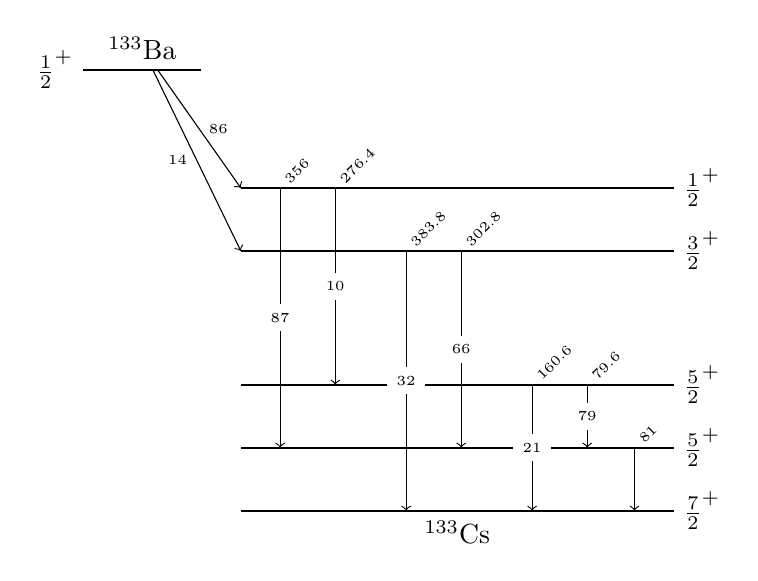
\begin{tikzpicture}
        \draw[thick]
        (-.5,5) node[left]{$\frac12^+$} -- node[above] (Ba) {${}^{133}$Ba} (1,5)
        (1.5,3.5) coordinate (EC1) -- (7,3.5) node[right] {$\frac12^+$}
        (1.5,2.7) coordinate (EC2) -- (7,2.7) node[right] {$\frac32^+$}
        (1.5,1.0)  -- (7,1.0) node[right] {$\frac52^+$}
        (1.5,0.2)  -- (7,0.2) node[right] {$\frac52^+$}
        (1.5,-0.6) -- node[below] {${}^{133}$Cs} (7,-0.6) node[right] {$\frac72^+$}
        ;
        \draw[->]
        (Ba) -- node[right]{\tiny{\SI{86}{\percent}}} (EC1)
        ;
        \draw[->]
        (Ba) -- node[left]{\tiny{\SI{14}{\percent}}} (EC2)
        ;
        % Linien
        \draw[->]
        (2,3.5) node[right, rotate=45]
        {\tiny{\SI{356}{\kilo\electronvolt}}} -- node[midway,
        fill=white] {\tiny{\SI{87}{\percent}}} (2,.2)
        ;
        \draw[->]
        (2.7,3.5) node[right, rotate=45]
        {\tiny{\SI{276.4}{\kilo\electronvolt}}} -- node[midway,
        fill=white] {\tiny{\SI{10}{\percent}}} (2.7,1.)
        ;
        \draw[->]
        (3.6,2.7) node[right, rotate=45]
        {\tiny{\SI{383.8}{\kilo\electronvolt}}} -- node[midway,
        fill=white] {\tiny{\SI{32}{\percent}}} (3.6,-.6)
        ;
        \draw[->]
        (4.3,2.7) node[right, rotate=45]
        {\tiny{\SI{302.8}{\kilo\electronvolt}}} -- node[midway,
        fill=white] {\tiny{\SI{66}{\percent}}} (4.3,.2)
        ;
        \draw[->]
        (5.2,1.0) node[right, rotate=45]
        {\tiny{\SI{160.6}{\kilo\electronvolt}}} -- node[midway,
        fill=white] {\tiny{\SI{21}{\percent}}} (5.2,-.6)
        ;
        \draw[->]
        (5.9,1.0) node[right, rotate=45]
        {\tiny{\SI{79.6}{\kilo\electronvolt}}} -- node[midway,
        fill=white] {\tiny{\SI{79}{\percent}}} (5.9,.2)
        ;
        \draw[->]
        (6.5,.2) node[right, rotate=45]
        {\tiny{\SI{81}{\kilo\electronvolt}}} -- (6.5,-.6)
        ;
    \end{tikzpicture}
    \caption{%
        Zerfallsschema von ${}^{133}$Ba. Übernommen aus \parencite{Ueding/525}.
    }
    \label{fig:Ba-Zerfall}
\end{figure}

% TODO Zerfallsschema 137Cs.

\chapter{Durchführung}

\section{Vorbereitung}

\section{Totaler Stoßwirkungsquerschnitt}

\section{Energiekalibrierung des Spektrometers}

\section{Messung der Streuspektren}

\chapter{Auswertung}

\chapter{Ergebnis}

% TODO Ergebnis.

\IfFileExists{\bibliographyfile}{
    \printbibliography
}{}

\end{document}

% vim: spell spelllang=de tw=79
